%% State Space Modelling of Dynamic Systems
%% Lecture 17: Transformation of States and Solution of State Equations
\def\FileDate{10/01/31}
\def\FileVersion{1.0}
% ----------------------------------------------------------------
% Notes pages *********************************************************
% ----------------------------------------------------------------


The canonical forms described in the last lecture give different descriptions of the same transfer function (TF) and are therefore equivalent in their overall input-output relationship. This means that it should be possible to convert one canonical form into another by the operation of simple matrix operations. Furthermore, by transforming a system to the \emph{normal form}, determining the response and mapping back, it is possible to determine the total system response of any state space system.

The \emph{eigenvalues} of the state matrix $\mathbf{A}$ have an important influence on the system response and understanding them is key to understanding the general solution of state-space systems.

In this lecture we define eigenvalues and eigenvectors, show the system transformation method and prove that it has no impact on the system eigenvalues, show how it can be used to transform an arbitrary state-space model into one with a diagonal (normal) structure, and finally we use these results to find a general time-response solution to the state space equations.

\ifslidesonly
\begin{slide}
   \heading{Transformation of State Models}
\begin{itemize}
	\item For a given transfer function the canonical forms are equivalent in their input-output relationships.
	\item We can convert one form of canonical system into another by the application of simple matrix operations.
	\item Transforming to normal form simplifies the calculation of system response.
	\item The \emph{eigenvalues} of the $\mathbf{A}$ matrix are key to the process.
	\item Knowledge of a system's eigenvalues means that we can determine the system response of any LTI system.
\end{itemize}   
\end{slide}
\begin{slide}
   \heading{Lecture Contents}
\begin{itemize}
	\item Eigenvalues and eigenvectors
	\item System transformation
	\item Diagonalization of a state space model
	\item Solution to the general state equations
\end{itemize}
\end{slide}
\fi

\section*{Eigenvalues and Eigenvectors} % (fold)
\label{sub:eigenvalues_and_eigenvectors}

\subsection*{Definitions} % (fold)
\label{ssub:Definitions}


\emph{Eigenvector}:\footnote{The world \emph{eigen} is from the German for ``characteristic'' so another name for eigenvalue might be \emph{characteristic value}. There is a very close relationship between the eigenvalues and the characteristic equation we have discussed in earlier lectures. Indeed as we shall see, the equation $\det(\lambda\mathbf{I}-\mathbf{A})=0$ that is used to find the eignenvalues of a system is almost identical to $\det(s\mathbf{I}-A)=0$ that determines the poles of the system defined in transfer function form. From this is should be clear that the eigenvalues of the $\mathbf{A}$ matrix are the same as the poles of the corresponding transfer function.} The vector $[v_{31}, i_{1}]^T$ is called the ``\emph{state
vector}.'' Its elements are state variables.
\endinput
%%% Local Variables: 
%%% mode: latex
%%% TeX-master: "notes"
%%% End: 

\ifslidesonly
\begin{slide}
   \heading{Definition of an Eigenvector}
   The vector $[v_{31}, i_{1}]^T$ is called the ``\emph{state
vector}.'' Its elements are state variables.
\endinput
%%% Local Variables: 
%%% mode: latex
%%% TeX-master: "notes"
%%% End: 

\end{slide}
\fi
\sref{slide:eigenvector} illustrates this definition of eigenvectors. If $\mathbf{Ax}$ is not collinear with $\mathbf{x}$ after the transformation, $\mathbf{x}$ is not an eigenvector. If $\mathbf{Ax}$ is collinear with $\mathbf{x}$ after the transformation, $\mathbf{x}$ is  an eigenvector.

\begin{slide}\label{slide:eigenvector}
   \heading{Eigenvectors and Transformations}
	\begin{center}
		\resizebox{280pt}{!}{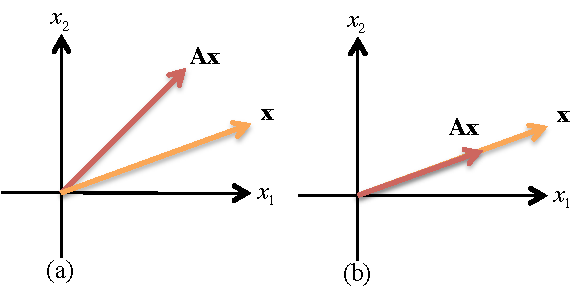
\includegraphics{pictures/eigenvectors.pdf}}
	\end{center}
   To be an eigenvector, the transformation $\mathbf{Ax}$ must be collinear with $\mathbf{x}$. Thus, in (a), $\mathbf{x}$ is not an eigenvector: in (b), it is.
\end{slide}

\emph{Eigenvalues}: The eigenvalues of the matrix $\mathbf{A}$ are the values of $\lambda_i$ that satisfy (\ref{eq:eigenvector}) for $\mathbf{x}_i\ne \mathbf{0}$.

To find the eigenvectors, we arrange equation (\ref{eq:eigenvector}). Eigenvectors, $\mathbf{x}_i$, satisfy
\begin{equation}\label{eq:581}
	\mathbf{0}=(\lambda_i\mathbf{I}-\mathbf{A})\mathbf{x}_i 
\end{equation}
Solving for $\mathbf{x}_i$ by premultiplying both sides by $(\lambda_i\mathbf{I}-\mathbf{A})^{-1}$ yields
\[
	\mathbf{x}_i = (\lambda_i\mathbf{I}-\mathbf{A})^{-1}\mathbf{0} = 
	       \frac{\textrm{adj}(\lambda_i\mathbf{I}-\mathbf{A})^{-1}}{\det(\lambda_i\mathbf{I}-\mathbf{A})^{-1}}\mathbf{0} 
\]
Since $\mathbf{x}_i\ne \mathbf{0}$, a nonzero solution exists if
\begin{equation}\label{eq:eigenvalue}
	\det(\lambda_i\mathbf{I}-\mathbf{A}) = \mathbf{0} \label{eq:eigenvalue}
\end{equation}
From which $\lambda_i$, the eigenvalues, can be found.
\ifslidesonly
\begin{slide}
   \heading{Eigenvalues}
The eigenvalues of the matrix $\mathbf{A}$ are the values of $\lambda_i$ that satisfy (\ref{eq:eigenvector}) for $\mathbf{x}_i\ne \mathbf{0}$.

The eigenvectors, $\mathbf{x}_i$, satisfy
\begin{equation}
	\mathbf{0}=(\lambda_i\mathbf{I}-\mathbf{A})\mathbf{x}_i \label{eq:581} 
\end{equation}
Solving for $\mathbf{x}_i$ (see notes), a nonzero solution exists if
\begin{equation}\label{eq:eigenvalue}
	\det(\lambda_i\mathbf{I}-\mathbf{A}) = \mathbf{0} \label{eq:eigenvalue}
\end{equation}   
From which $\lambda_i$, the eigenvalues, can be found.
\end{slide}
\fi

We are now ready to show how to find the eigenvectors $\mathbf{x}_i$. First we find the eigenvalues, $\lambda_i$, using $\det(\lambda_i\mathbf{I}-\mathbf{A} = \mathbf{0})$, and then we use equation (\ref{eq:eigenvector}) to find the eigenvectors.

\ifslidesonly
\begin{slide}
   \heading{Finding the eigenvectors of a system}
   To find the eigenvectors $\mathbf{x}_i$ of a system matrix $\mathbf{A}$
\begin{enumerate}
   	\item First find the eigenvalues, $\lambda_i$, using $\det(\lambda_i\mathbf{I}-\mathbf{A} = \mathbf{0})$
   	\item Use $\mathbf{A}\mathbf{x}_i=\lambda_i\mathbf{x}_i$ to find the eigenvectors.
   \end{enumerate}
   See the worked example in the notes.
\end{slide}
\fi

\subsection*{Example 1: finding eigenvectors} % (fold)
\label{ssub:example_1}

\textbf{Problem}: Find the eigenvectors of the matrix
\begin{equation}
	{\bf{A}} = \left[ {\begin{array}{*{20}c}
	   { - 3} & 1  \\
	   1 & { - 3}  \\
	\end{array}} \right]
\end{equation}

\textbf{SOLUTION}: The eigenvectors, $\mathbf{x}_i$, satisfy Eq. (\ref{eq:581}). First, use $\det(\lambda_i\mathbf{I}-\mathbf{A})=0$ to find the eigenvalues, $\lambda_i$, for Eq. (\ref{eq:581}):
% MathType!MTEF!2!1!+-
% faaagaart1ev2aaaKnaaaaWenf2ys9wBH5garuavP1wzZbqedmvETj
% 2BSbqefm0B1jxALjharqqtubsr4rNCHbGeaGqiVu0Je9sqqrpepC0x
% bbL8FesqqrFfpeea0xe9Lq-Jc9vqaqpepm0xbba9pwe9Q8fs0-yqaq
% pepae9pg0FirpepeKkFr0xfr-xfr-xb9Gqpi0dc9adbaqaaeGaciGa
% aiaabeqaamaabaabaaGceaabbeaaciGGKbGaaiyzaiaacshacaGGOa
% Gaeq4UdWMaaCysaiabgkHiTiaahgeacaGGPaGaeyypa0ZaaqWaaeaa
% daWadaqaauaadeqaciaaaeaacqaH7oaBaeaacaaIWaaabaGaaGimaa
% qaaiabeU7aSbaaaiaawUfacaGLDbaacqGHsisldaWadaqaauaadeqa
% ciaaaeaacqGHsislcaaIZaaabaGaaGymaaqaaiaaigdaaeaacqGHsi
% slcaaIZaaaaaGaay5waiaaw2faaaGaay5bSlaawIa7aaqaaiabg2da
% 9maaemaabaqbamqabiGaaaqaaiabeU7aSjabgUcaRiaaiodaaeaacq
% GHsislcaaIXaaabaGaeyOeI0IaaGymaaqaaiabeU7aSjabgUcaRiaa
% iodaaaaacaGLhWUaayjcSdaabaGaeyypa0Jaeq4UdW2aaWbaaSqabe
% aacaaIYaaaaOGaey4kaSIaaGOnaiabeU7aSjabgUcaRiaaiIdaaaaa
% !6018!
\[
\begin{array}{c}
 \det (\lambda {\bf{I}} - {\bf{A}}) = \left| {\left[ {\begin{array}{*{20}c}
   \lambda  & 0  \\
   0 & \lambda   \\
\end{array}} \right] - \left[ {\begin{array}{*{20}c}
   { - 3} & 1  \\
   1 & { - 3}  \\
\end{array}} \right]} \right| \\ 
  = \left| {\begin{array}{*{20}c}
   {\lambda  + 3} & { - 1}  \\
   { - 1} & {\lambda  + 3}  \\
\end{array}} \right| \\ 
  = \lambda ^2  + 6\lambda  + 8 \\ 
 \end{array}
\]

from which the eigenvalues are $\lambda_1 = -2$ and $\lambda_2 = -4$. 

Using Eq. (\ref{eq:eigenvector}) successively with each eigenvalue, we have
% MathType!MTEF!2!1!+-
% faaagaart1ev2aaaKnaaaaWenf2ys9wBH5garuavP1wzZbqedmvETj
% 2BSbqefm0B1jxALjharqqtubsr4rNCHbGeaGqiVu0Je9sqqrpepC0x
% bbL8FesqqrFfpeea0xe9Lq-Jc9vqaqpepm0xbba9pwe9Q8fs0-yqaq
% pepae9pg0FirpepeKkFr0xfr-xfr-xb9Gqpi0dc9adbaqaaeGaciGa
% aiaabeqaamaabaabaaGceaqabeaacaWHbbGaaCiEamaaBaaaleaaca
% WGPbaabeaakiabg2da9iabeU7aSjaahIhadaWgaaWcbaGaamyAaaqa
% baaakeaadaWadaqaauaadeqaciaaaeaacqGHsislcaaIZaaabaGaaG
% ymaaqaaiaaigdaaeaacqGHsislcaaIZaaaaaGaay5waiaaw2faamaa
% dmaabaqbamqabiqaaaqaaiaadIhadaWgaaWcbaGaaGymaaqabaaake
% aacaWG4bWaaSbaaSqaaiaaikdaaeqaaaaaaOGaay5waiaaw2faaiab
% g2da9iabgkHiTiaaikdadaWadaqaauaadeqaceaaaeaacaWG4bWaaS
% baaSqaaiaaigdaaeqaaaGcbaGaamiEamaaBaaaleaacaaIYaaabeaa
% aaaakiaawUfacaGLDbaaaaaa!4B20!
\[
\begin{array}{l}
 {\bf{Ax}}_i  = \lambda {\bf{x}}_i  \\ 
 \left[ {\begin{array}{*{20}c}
   { - 3} & 1  \\
   1 & { - 3}  \\
\end{array}} \right]\left[ {\begin{array}{*{20}c}
   {x_1 }  \\
   {x_2 }  \\
\end{array}} \right] =  - 2\left[ {\begin{array}{*{20}c}
   {x_1 }  \\
   {x_2 }  \\
\end{array}} \right] \\ 
 \end{array}
\]
or
\begin{eqnarray*}
-3x_1+x_2 & = & -2x_1 \\
x_1-3x_2 & = & -2x_2
\end{eqnarray*}
from which $x_1 = x_2$. Thus,
% MathType!MTEF!2!1!+-
% faaagaart1ev2aaaKnaaaaWenf2ys9wBH5garuavP1wzZbqedmvETj
% 2BSbqefm0B1jxALjharqqtubsr4rNCHbGeaGqiVu0Je9sqqrpepC0x
% bbL8FesqqrFfpeea0xe9Lq-Jc9vqaqpepm0xbba9pwe9Q8fs0-yqaq
% pepae9pg0FirpepeKkFr0xfr-xfr-xb9Gqpi0dc9adbaqaaeGaciGa
% aiaabeqaamaabaabaaGcbaGaaCiEaiabg2da9maadmaabaqbamqabi
% qaaaqaaiaadogaaeaacaWGJbaaaaGaay5waiaaw2faaaaa!33EA!
\begin{equation}\label{ex1:ev1}
{\bf{x}} = \left[ {\begin{array}{*{20}c}
   c  \\
   c  \\
\end{array}} \right]
\end{equation}
Using the other eigenvalue, $-4$, we have
\begin{equation}\label{ex1:ev2}
{\bf{x}} = \left[ {\begin{array}{*{20}c}
   c  \\
   -c  \\
\end{array}} \right]
\end{equation}
Using Eqs. (\ref{ex1:ev1}) and (\ref{ex1:ev2}), one choice of eigenvectors is
% MathType!MTEF!2!1!+-
% faaagaart1ev2aaaKnaaaaWenf2ys9wBH5garuavP1wzZbqedmvETj
% 2BSbqefm0B1jxALjharqqtubsr4rNCHbGeaGqiVu0Je9sqqrpepC0x
% bbL8FesqqrFfpeea0xe9Lq-Jc9vqaqpepm0xbba9pwe9Q8fs0-yqaq
% pepae9pg0FirpepeKkFr0xfr-xfr-xb9Gqpi0dc9adbaqaaeGaciGa
% aiaabeqaamaabaabaaGcbaGaaCiEamaaBaaaleaacaaIXaaabeaaki
% abg2da9maadmaabaqbamqabiqaaaqaaiaaigdaaeaacaaIXaaaaaGa
% ay5waiaaw2faaiaaywW7caqGHbGaaeOBaiaabsgacaaMf8UaaCiEam
% aaBaaaleaacaaIYaaabeaakiabg2da9maadmaabaqbamqabiqaaaqa
% aiaaigdaaeaacqGHsislcaaIXaaaaaGaay5waiaaw2faaaaa!41B6!
\begin{equation}\label{ex1:solution}
{\bf{x}}_1  = \left[ {\begin{array}{*{20}c}
   1  \\
   1  \\
\end{array}} \right]\quad {\rm{and}}\quad {\bf{x}}_2  = \left[ {\begin{array}{*{20}c}
   1  \\
   { - 1}  \\
\end{array}} \right]
\end{equation}


% subsection example_1 (end)

% section eigenvalues_and_eigenvectors (end)

\section*{Transformation of State Space Models}



\begin{center}
	\resizebox{200pt}{!}{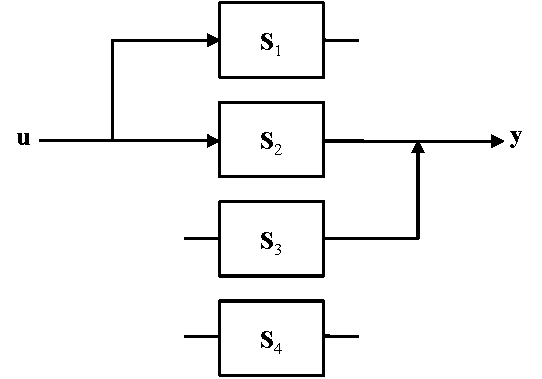
\includegraphics{pictures/partitioning.pdf}}
\end{center}
\endinput

%%% Local Variables: 
%%% mode: latex
%%% TeX-master: "notes"
%%% End:
\ifslidesonly
\begin{slide}
	\heading{State Transformation}
   
\begin{center}
	\resizebox{200pt}{!}{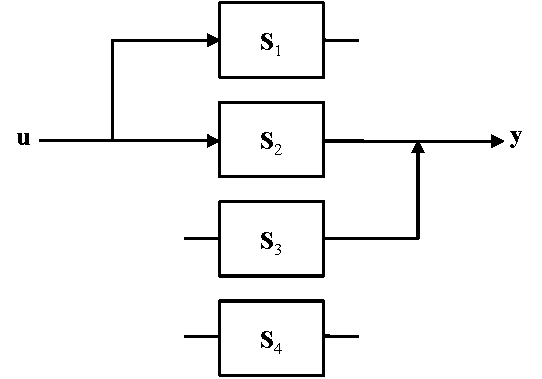
\includegraphics{pictures/partitioning.pdf}}
\end{center}
\endinput

%%% Local Variables: 
%%% mode: latex
%%% TeX-master: "notes"
%%% End:
\end{slide}
\fi

Given the transformation $\mathbf{T}^{-1}\mathbf{AT}=\mathbf{\Lambda}$:
\begin{eqnarray*}
	\mathbf{A}t & = & (\mathbf{T\Lambda T}^{-1}) t \\
	\mathbf{A}^nt^n & = & (\mathbf{T\Lambda T}^{-1})(\mathbf{T\Lambda T}^{-1})\ldots(\mathbf{T\Lambda T}^{-1})t^n \\
	                & = & \mathbf{T\Lambda T}^{-1}\mathbf{T\Lambda T}^{-1}\ldots\mathbf{T\Lambda T}^{-1}t^n \\
	\mathbf{A}^nt^n & = & \mathbf{T\Lambda}\mathbf{I}\mathbf{\Lambda I}\ldots\mathbf{I\Lambda T}^{-1}t^n \\
	\               & = & \mathbf{T\Lambda}^n\mathbf{T}^{-1}t^n \\
\end{eqnarray*}
\endinput

%%% Local Variables: 
%%% mode: latex
%%% TeX-master: "notes"
%%% End:
\ifslidesonly
\begin{slide}
	\heading{Output Transformation}
   Given the transformation $\mathbf{T}^{-1}\mathbf{AT}=\mathbf{\Lambda}$:
\begin{eqnarray*}
	\mathbf{A}t & = & (\mathbf{T\Lambda T}^{-1}) t \\
	\mathbf{A}^nt^n & = & (\mathbf{T\Lambda T}^{-1})(\mathbf{T\Lambda T}^{-1})\ldots(\mathbf{T\Lambda T}^{-1})t^n \\
	                & = & \mathbf{T\Lambda T}^{-1}\mathbf{T\Lambda T}^{-1}\ldots\mathbf{T\Lambda T}^{-1}t^n \\
	\mathbf{A}^nt^n & = & \mathbf{T\Lambda}\mathbf{I}\mathbf{\Lambda I}\ldots\mathbf{I\Lambda T}^{-1}t^n \\
	\               & = & \mathbf{T\Lambda}^n\mathbf{T}^{-1}t^n \\
\end{eqnarray*}
\endinput

%%% Local Variables: 
%%% mode: latex
%%% TeX-master: "notes"
%%% End:
\end{slide}
\fi

The matrix function becomes:
\begin{eqnarray*}
	f(\mathbf{A}t) & = & f_0\mathbf{TIT}^{-1} + f_1\mathbf{T\Lambda T}^{-1}t + f_2\mathbf{T\Lambda}^2\mathbf{T}^{-1}t^2 + \cdots + f_n\mathbf{T\Lambda}^n\mathbf{T}^{-1}t^n + \cdots \\
	f(\mathbf{A}t) & = & \mathbf{T}\left(f_0\mathbf{I} + f_1\mathbf{\Lambda}t + f_2\mathbf{\Lambda}^2t^2 + \cdots + f_n\mathbf{\Lambda}^nt^n + \cdots \right)\mathbf{T}^{-1}\\
	               & = & \mathbf{T}f(\mathbf{\Lambda}t)\mathbf{T}^{-1}
\end{eqnarray*}
 
The term inside the brackets on the rhs is a diagonal matrix and the $i^\mathrm{th}$ diagonal element is:
\[
f_0+f_1\lambda_it + f_2\lambda_i^2t^2 + \cdots + f_n\lambda_i^nt^ + \cdots
\]
From the Taylor series this must be $f(\lambda_i t)$:
\[
f(\mathbf{A} t)=\mathbf{T} f(\mathbf{\Lambda} t) \mathbf{T}^{-1}
\]   
where $f(\mathbf{\Lambda} t)=\mathrm{diag}\left(f(\lambda_i t)\right)$.

\endinput

%%% Local Variables: 
%%% mode: latex
%%% TeX-master: "notes"
%%% End:
\ifslidesonly
\begin{slide}
	\heading{Transformed Model}
   The matrix function becomes:
\begin{eqnarray*}
	f(\mathbf{A}t) & = & f_0\mathbf{TIT}^{-1} + f_1\mathbf{T\Lambda T}^{-1}t + f_2\mathbf{T\Lambda}^2\mathbf{T}^{-1}t^2 + \cdots + f_n\mathbf{T\Lambda}^n\mathbf{T}^{-1}t^n + \cdots \\
	f(\mathbf{A}t) & = & \mathbf{T}\left(f_0\mathbf{I} + f_1\mathbf{\Lambda}t + f_2\mathbf{\Lambda}^2t^2 + \cdots + f_n\mathbf{\Lambda}^nt^n + \cdots \right)\mathbf{T}^{-1}\\
	               & = & \mathbf{T}f(\mathbf{\Lambda}t)\mathbf{T}^{-1}
\end{eqnarray*}
 
The term inside the brackets on the rhs is a diagonal matrix and the $i^\mathrm{th}$ diagonal element is:
\[
f_0+f_1\lambda_it + f_2\lambda_i^2t^2 + \cdots + f_n\lambda_i^nt^ + \cdots
\]
From the Taylor series this must be $f(\lambda_i t)$:
\[
f(\mathbf{A} t)=\mathbf{T} f(\mathbf{\Lambda} t) \mathbf{T}^{-1}
\]   
where $f(\mathbf{\Lambda} t)=\mathrm{diag}\left(f(\lambda_i t)\right)$.

\endinput

%%% Local Variables: 
%%% mode: latex
%%% TeX-master: "notes"
%%% End:
\end{slide}
\fi

\begin{itemize}
	\item Notice that the state matrix $\mathbf{A}'$for the new model is a \emph{similarity transformation} on the $\mathbf{A}$ matrix of the original system and therefore they share the same set of eigenvalues.
	\item This should not be surprising since the poles of the system being modelled correspond to the eigenvalues of the state matrix, whatever the choice of states.
\end{itemize}



\subsection*{Proof} % (fold)
\label{sub:invariance_of_system_transformation}

From previous work the error dynamics are:
\[
\dot{\mathbf{e}} = (\mathbf{A}-\mathbf{LC})\mathbf{e}
\]
Therefore the dynamics of the combined system is:
\[\left[ {\begin{array}{*{20}c}
   {\dot{\mathbf{x}}}  \\
   {\dot{\mathbf{e}}ß}  \\
\end{array}} \right] = \left[ {\begin{array}{*{20}c}
   {\left( {{\bf{A}} - {\bf{BK}}} \right)} & {{\bf{BK}}}  \\
   {\bf{0}} & {\left( {{\bf{A}} - {\bf{LC}}} \right)}  \\
\end{array}} \right]\left[ {\begin{array}{*{20}c}
   {\bf{x}}  \\
   {\bf{e}}  \\
\end{array}} \right] + \left[ {\begin{array}{*{20}c}
   {\bf{B}}  \\
   {\bf{0}}  \\
\end{array}} \right]r
\]
\endinput

%%% Local Variables: 
%%% mode: latex
%%% TeX-master: "notes"
%%% End:
\ifslidesonly
\begin{slide}
	\heading{Similarity Transform Preserves Eigenvalues}
	The transformation $\mathbf{T}^{-1}\mathbf{AT}$ is a \emph{similarity transform}. That is the eigenvalues are the same as for $\mathbf{A}$.
	
\emph{Proof}
   From previous work the error dynamics are:
\[
\dot{\mathbf{e}} = (\mathbf{A}-\mathbf{LC})\mathbf{e}
\]
Therefore the dynamics of the combined system is:
\[\left[ {\begin{array}{*{20}c}
   {\dot{\mathbf{x}}}  \\
   {\dot{\mathbf{e}}ß}  \\
\end{array}} \right] = \left[ {\begin{array}{*{20}c}
   {\left( {{\bf{A}} - {\bf{BK}}} \right)} & {{\bf{BK}}}  \\
   {\bf{0}} & {\left( {{\bf{A}} - {\bf{LC}}} \right)}  \\
\end{array}} \right]\left[ {\begin{array}{*{20}c}
   {\bf{x}}  \\
   {\bf{e}}  \\
\end{array}} \right] + \left[ {\begin{array}{*{20}c}
   {\bf{B}}  \\
   {\bf{0}}  \\
\end{array}} \right]r
\]
\endinput

%%% Local Variables: 
%%% mode: latex
%%% TeX-master: "notes"
%%% End:
\end{slide}
\fi

Therefore if $\lambda$ is an eigenvalue of $\mathbf{A}$ the it is also one of $\mathbf{A}'=\mathbf{T}^{-1}\mathbf{AT}$. 

\emph{QED}.

% subsection invariance_of_system_transformation (end)

\subsection*{Example 2: Similarity transformations on state equations}
\label{sub:similarity_transforms_on_state_equations}

\textbf{Problem}: Given the system represented in state space by the following equations
% MathType!MTEF!2!1!+-
% faaagaart1ev2aaaKnaaaaWenf2ys9wBH5garuavP1wzZbqedmvETj
% 2BSbqefm0B1jxALjharqqtubsr4rNCHbGeaGqiVu0Je9sqqrpepC0x
% bbL8FesqqrFfpeea0xe9Lq-Jc9vqaqpepm0xbba9pwe9Q8fs0-yqaq
% pepae9pg0FirpepeKkFr0xfr-xfr-xb9Gqpi0dc9adbaqaaeGaciGa
% aiaabeqaamaabaabaaGceaqabeaaceWH4bGbaiaacqGH9aqpdaWada
% qaauaadeqadmaaaeaacaaIWaaabaGaaGymaaqaaiaaicdaaeaacaaI
% WaaabaGaaGimaaqaaiaaigdaaeaacqGHsislcaaIYaaabaGaeyOeI0
% IaaGynaaqaaiabgkHiTiaaiEdaaaaacaGLBbGaayzxaaGaaCiEaiab
% gUcaRmaadmaabaqbamqabmqaaaqaaiaaicdaaeaacaaIWaaabaGaaG
% ymaaaaaiaawUfacaGLDbaacaWG1baabaGaamyEaiabg2da9maadmaa
% baqbamqabeWaaaqaaiaaigdaaeaacaaIWaaabaGaaGimaaaaaiaawU
% facaGLDbaacaWH4baaaaa!49DB!
\[
\begin{array}{l}
 {\bf{\dot x}} = \left[ {\begin{array}{*{20}c}
   0 & 1 & 0  \\
   0 & 0 & 1  \\
   { - 2} & { - 5} & { - 7}  \\
\end{array}} \right]{\bf{x}} + \left[ {\begin{array}{*{20}c}
   0  \\
   0  \\
   1  \\
\end{array}} \right]u \\ 
 y = \left[ {\begin{array}{*{20}c}
   1 & 0 & 0  \\
\end{array}} \right]{\bf{x}} \\ 
 \end{array}
\]
transform the system to a new set of state variables, $\mathbf{w}$, where the new state variables are related to the original state variables, $\mathbf{x}$, as follows:
\begin{eqnarray*}
	w_1 & = & 2x_1 \\
	w_2 & = & 3x_1 + 2x_2 \\
	w_3 & = & x_1 + 4x_2 + 5x_3
\end{eqnarray*}

\textbf{SOLUTION}: Expressing the transformed states in vector-matrix form,
% MathType!MTEF!2!1!+-
% faaagaart1ev2aaaKnaaaaWenf2ys9wBH5garuavP1wzZbqedmvETj
% 2BSbqefm0B1jxALjharqqtubsr4rNCHbGeaGqiVu0Je9sqqrpepC0x
% bbL8FesqqrFfpeea0xe9Lq-Jc9vqaqpepm0xbba9pwe9Q8fs0-yqaq
% pepae9pg0FirpepeKkFr0xfr-xfr-xb9Gqpi0dc9adbaqaaeGaciGa
% aiaabeqaamaabaabaaGcbaGaaC4Daiabg2da9maadmaabaqbamqabm
% WaaaqaaiaaikdaaeaacaaIWaaabaGaaGimaaqaaiaaiodaaeaacaaI
% YaaabaGaaGimaaqaaiaaigdaaeaacaaI0aaabaGaaGynaaaaaiaawU
% facaGLDbaacaWH4bGaeyypa0JaaCivamaaCaaaleqabaGaeyOeI0Ia
% aGymaaaakiaahIhaaaa!3E82!
\[
{\bf{w}} = \left[ {\begin{array}{*{20}c}
   2 & 0 & 0  \\
   3 & 2 & 0  \\
   1 & 4 & 5  \\
\end{array}} \right]{\bf{x}} = {\bf{T}}^{ - 1} {\bf{x}}
\]

Thus
% MathType!MTEF!2!1!+-
% faaagaart1ev2aaaKnaaaaWenf2ys9wBH5garuavP1wzZbqedmvETj
% 2BSbqefm0B1jxALjharqqtubsr4rNCHbGeaGqiVu0Je9sqqrpepC0x
% bbL8FesqqrFfpeea0xe9Lq-Jc9vqaqpepm0xbba9pwe9Q8fs0-yqaq
% pepae9pg0FirpepeKkFr0xfr-xfr-xb9Gqpi0dc9adbaqaaeGaciGa
% aiaabeqaamaabaabaaGceaabbeaacaWHubWaaWbaaSqabeaacqGHsi
% slcaaIXaaaaOGaaCyqaiaahsfacqGH9aqpdaWadaqaauaadeqadmaa
% aeaacaaIYaaabaGaaGimaaqaaiaaicdaaeaacaaIZaaabaGaaGOmaa
% qaaiaaicdaaeaacaaIXaaabaGaaGinaaqaaiaaiwdaaaaacaGLBbGa
% ayzxaaGaaGjbVpaadmaabaqbamqabmWaaaqaaiaaicdaaeaacaaIXa
% aabaGaaGimaaqaaiaaicdaaeaacaaIWaaabaGaaGymaaqaaiabgkHi
% TiaaikdaaeaacqGHsislcaaI1aaabaGaeyOeI0IaaG4naaaaaiaawU
% facaGLDbaacaaMe8+aamWaaeaafaWabeWadaaabaGaaGimaiaac6ca
% caaI1aaabaGaaGimaaqaaiaaicdaaeaacqGHsislcaaIWaGaaiOlai
% aaiEdacaaI1aaabaGaaGimaiaac6cacaaI1aaabaGaaGimaaqaaiaa
% icdacaGGUaGaaGynaaqaaiabgkHiTiaaicdacaGGUaGaaGinaaqaai
% aaicdacaGGUaGaaGOmaaaaaiaawUfacaGLDbaaaeaacqGH9aqpdaWa
% daqaauaadeqadmaaaeaacqGHsislcaaIXaGaaiOlaiaaiwdaaeaaca
% aIXaaabaGaaGimaaqaaiabgkHiTiaaigdacaGGUaGaaGOmaiaaiwda
% aeaacaaIWaGaaiilaiaaiEdaaeaacaaIWaGaaiOlaiaaisdaaeaacq
% GHsislcaaIYaGaaiOlaiaaiwdaaeaacaaIWaGaaiOlaiaaisdaaeaa
% cqGHsislcaaI2aGaaiOlaiaaikdaaaaacaGLBbGaayzxaaaaaaa!76AB!
\[
\begin{array}{c}
 {\bf{T}}^{ - 1} {\bf{AT}} = \left[ {\begin{array}{*{20}c}
   2 & 0 & 0  \\
   3 & 2 & 0  \\
   1 & 4 & 5  \\
\end{array}} \right]\;\left[ {\begin{array}{*{20}c}
   0 & 1 & 0  \\
   0 & 0 & 1  \\
   { - 2} & { - 5} & { - 7}  \\
\end{array}} \right]\;\left[ {\begin{array}{*{20}c}
   {0.5} & 0 & 0  \\
   { - 0.75} & {0.5} & 0  \\
   {0.5} & { - 0.4} & {0.2}  \\
\end{array}} \right] \\ 
  = \left[ {\begin{array}{*{20}c}
   { - 1.5} & 1 & 0  \\
   { - 1.25} & {0.7} & {0.4}  \\
   { - 2.5} & {0.4} & { - 6.2}  \\
\end{array}} \right] \\ 
 \end{array}
\]

% MathType!MTEF!2!1!+-
% faaagaart1ev2aaaKnaaaaWenf2ys9wBH5garuavP1wzZbqedmvETj
% 2BSbqefm0B1jxALjharqqtubsr4rNCHbGeaGqiVu0Je9sqqrpepC0x
% bbL8FesqqrFfpeea0xe9Lq-Jc9vqaqpepm0xbba9pwe9Q8fs0-yqaq
% pepae9pg0FirpepeKkFr0xfr-xfr-xb9Gqpi0dc9adbaqaaeGaciGa
% aiaabeqaamaabaabaaGcbaGaaCivamaaCaaaleqabaGaeyOeI0IaaG
% ymaaaakiaahkeacqGH9aqpdaWadaqaauaadeqadmaaaeaacaaIYaaa
% baGaaGimaaqaaiaaicdaaeaacaaIZaaabaGaaGOmaaqaaiaaicdaae
% aacaaIXaaabaGaaGinaaqaaiaaiwdaaaaacaGLBbGaayzxaaGaaGjb
% VpaadmaabaqbamqabmqaaaqaaiaaicdaaeaacaaIWaaabaGaaGymaa
% aaaiaawUfacaGLDbaacqGH9aqpdaWadaqaauaadeqadeaaaeaacaaI
% WaaabaGaaGimaaqaaiaaiwdaaaaacaGLBbGaayzxaaaaaa!4640!
\[
{\bf{T}}^{ - 1} {\bf{B}} = \left[ {\begin{array}{*{20}c}
   2 & 0 & 0  \\
   3 & 2 & 0  \\
   1 & 4 & 5  \\
\end{array}} \right]\;\left[ {\begin{array}{*{20}c}
   0  \\
   0  \\
   1  \\
\end{array}} \right] = \left[ {\begin{array}{*{20}c}
   0  \\
   0  \\
   5  \\
\end{array}} \right]
\]

% MathType!MTEF!2!1!+-
% faaagaart1ev2aaaKnaaaaWenf2ys9wBH5garuavP1wzZbqedmvETj
% 2BSbqefm0B1jxALjharqqtubsr4rNCHbGeaGqiVu0Je9sqqrpepC0x
% bbL8FesqqrFfpeea0xe9Lq-Jc9vqaqpepm0xbba9pwe9Q8fs0-yqaq
% pepae9pg0FirpepeKkFr0xfr-xfr-xb9Gqpi0dc9adbaqaaeGaciGa
% aiaabeqaamaabaabaaGcbaGaaC4qaiaahsfacqGH9aqpdaWadaqaau
% aadeqabmaaaeaacaaIXaaabaGaaGimaaqaaiaaicdaaaaacaGLBbGa
% ayzxaaGaaGjbVpaadmaabaqbamqabmWaaaqaaiaaicdacaGGUaGaaG
% ynaaqaaiaaicdaaeaacaaIWaaabaGaeyOeI0IaaGimaiaac6cacaaI
% 3aGaaGynaaqaaiaaicdacaGGUaGaaGynaaqaaiaaicdaaeaacaaIWa
% GaaiOlaiaaiwdaaeaacqGHsislcaaIWaGaaiOlaiaaisdaaeaacaaI
% WaGaaiOlaiaaikdaaaaacaGLBbGaayzxaaGaeyypa0ZaamWaaeaafa
% WabeqadaaabaGaaGimaiaac6cacaaI1aaabaGaaGimaaqaaiaaicda
% aaaacaGLBbGaayzxaaaaaa!50FA!
\[
{\bf{CT}} = \left[ {\begin{array}{*{20}c}
   1 & 0 & 0  \\
\end{array}} \right]\;\left[ {\begin{array}{*{20}c}
   {0.5} & 0 & 0  \\
   { - 0.75} & {0.5} & 0  \\
   {0.5} & { - 0.4} & {0.2}  \\
\end{array}} \right] = \left[ {\begin{array}{*{20}c}
   {0.5} & 0 & 0  \\
\end{array}} \right]
\]

Therefore the transformed system is
% MathType!MTEF!2!1!+-
% faaagaart1ev2aaaKnaaaaWenf2ys9wBH5garuavP1wzZbqedmvETj
% 2BSbqefm0B1jxALjharqqtubsr4rNCHbGeaGqiVu0Je9sqqrpepC0x
% bbL8FesqqrFfpeea0xe9Lq-Jc9vqaqpepm0xbba9pwe9Q8fs0-yqaq
% pepae9pg0FirpepeKkFr0xfr-xfr-xb9Gqpi0dc9adbaqaaeGaciGa
% aiaabeqaamaabaabaaGceaqabeaaceWH3bGbaiaacqGH9aqpdaWada
% qaauaadeqadmaaaeaacqGHsislcaaIXaGaaiOlaiaaiwdaaeaacaaI
% XaaabaGaaGimaaqaaiabgkHiTiaaigdacaGGUaGaaGOmaiaaiwdaae
% aacaaIWaGaaiOlaiaaiEdaaeaacaaIWaGaaiOlaiaaisdaaeaacqGH
% sislcaaIYaGaaiOlaiaaiwdaaeaacqGHsislcaaIWaGaaiOlaiaais
% daaeaacaaIWaGaaiOlaiaaikdaaaaacaGLBbGaayzxaaGaaC4Daiab
% gUcaRmaadmaabaqbamqabmqaaaqaaiaaicdaaeaacaaIWaaabaGaaG
% ynaaaaaiaawUfacaGLDbaacaWG1baabaGaamyEaiabg2da9maadmaa
% baqbamqabeWaaaqaaiaaicdacaGGUaGaaGynaaqaaiaaicdaaeaaca
% aIWaaaaaGaay5waiaaw2faaiaahEhaaaaa!56FE!
\[
\begin{array}{l}
 {\bf{\dot w}} = \left[ {\begin{array}{*{20}c}
   { - 1.5} & 1 & 0  \\
   { - 1.25} & {0.7} & {0.4}  \\
   { - 2.5} & { - 0.4} & {0.2}  \\
\end{array}} \right]{\bf{w}} + \left[ {\begin{array}{*{20}c}
   0  \\
   0  \\
   5  \\
\end{array}} \right]u \\ 
 y = \left[ {\begin{array}{*{20}c}
   {0.5} & 0 & 0  \\
\end{array}} \right]{\bf{w}} \\ 
 \end{array}
\]


% subsection similarity_transforms_on_state_equations (end)
 
\section*{Diagonalization of a System Matrix} % (fold)
\label{sec:diagonalization_of_a_system_matrix}

If we choose the eigenvectors of a system matrix $\mathbf{A}$ to be the basis of a transformation, $\mathbf{T}$, the resulting system matrix will be in the diagonal normal form. Let the transformation matrix $\mathbf{T}$ consist of the eigenvectors of $\mathbf{A}$, $\mathbf{x}_i$.
\begin{equation}\label{eq:591}
	\mathbf{T}=[\mathbf{x}_1, \mathbf{x}_2, \mathbf{x}_3, \ldots, \mathbf{x}_n] 
\end{equation}
Since $\mathbf{x}_i$ are eigenvectors, $\mathbf{A}\mathbf{x}_i=\lambda_i\mathbf{x}_i$, which can be written equivalently as a set of equations expressed by
\begin{equation}\label{eq:592}
	\mathbf{AT}=\mathbf{T\Lambda}
\end{equation}
where $\mathbf{\Lambda}$ is a matrix which has the eigenvalues $\lambda_i$ on the diagonal in some order and zeros elsewhere, and $\mathbf{T}$ is as defined in Eq. (\ref{eq:591}). Solving Eq. (\ref{eq:592}) for $\mathbf{\Lambda}$ by premultiplying by $\mathbf{T}^{-1}$, we get
\begin{equation}\label{eq:593}
	\mathbf{\Lambda}=\mathbf{T}^{-1}\mathbf{AT} 
\end{equation}
which is the system matrix in normal canonical form.\footnote{Note we need to perform some additional manipulations if there are repeated or complex eigenvalues. We leave the discovery of these extra steps as an exercise for the interested student. It will not be examined!}
\ifslidesonly
\begin{slide}
   \heading{To Diagonalize a State Space Model}
   Choose the eigenvectors of a system matrix $\mathbf{A}$ to be the basis of a transformation $\mathbf{T}$.
\begin{equation}\label{eq:591}
	\mathbf{T}=[\mathbf{x}_1, \mathbf{x}_2, \mathbf{x}_3, \ldots, \mathbf{x}_n] 
\end{equation}
$\mathbf{A}\mathbf{x}_i=\lambda_i\mathbf{x}_i$, can be written equivalently as a set of equations expressed by
\begin{equation}\label{eq:592}
	\mathbf{AT}=\mathbf{T\Lambda}
\end{equation}
Solving Eq. (\ref{eq:592}) for $\mathbf{\Lambda}$
\begin{equation}\label{eq:593}
	\mathbf{\Lambda}=\mathbf{T}^{-1}\mathbf{AT} 
\end{equation}
which is the system matrix in normal canonical form.
\end{slide}
\fi
In summary, under the transformation $\mathbf{T}$, consisting of the eigenvalues of the system matrix, the transformed system is identical to that obtained using the partial fraction expansion of the transfer function with distinct real roots. 
% section diagonalization_of_a_system_matrix (end)

\subsection*{Example 3: Diagonalization of a system in state space} % (fold)
\label{ssub:example_2}

\textbf{Problem}: Give the system shown below, find the diagonal (normal form) system that is similar.
% MathType!MTEF!2!1!+-
% faaagaart1ev2aaaKnaaaaWenf2ys9wBH5garuavP1wzZbqedmvETj
% 2BSbqefm0B1jxALjharqqtubsr4rNCHbGeaGqiVu0Je9sqqrpepC0x
% bbL8FesqqrFfpeea0xe9Lq-Jc9vqaqpepm0xbba9pwe9Q8fs0-yqaq
% pepae9pg0FirpepeKkFr0xfr-xfr-xb9Gqpi0dc9adbaqaaeGaciGa
% aiaabeqaamaabaabaaGceaabbeaaceWH4bGbaiaacqGH9aqpdaWada
% qaauaadeqaciaaaeaacqGHsislcaaIZaaabaGaaGymaaqaaiaaigda
% aeaacqGHsislcaaIZaaaaaGaay5waiaaw2faaiaahIhacqGHRaWkda
% WadaqaauaadeqaceaaaeaacaaIXaaabaGaaGOmaaaaaiaawUfacaGL
% DbaacaWG1baabaGaamyEaiabg2da9maadmaabaqbamqabeGaaaqaai
% aaikdaaeaacaaIZaaaaaGaay5waiaaw2faaiaahIhaaaaa!43CE!
\[
\begin{array}{c}
 {\bf{\dot x}} = \left[ {\begin{array}{*{20}c}
   { - 3} & 1  \\
   1 & { - 3}  \\
\end{array}} \right]{\bf{x}} + \left[ {\begin{array}{*{20}c}
   1  \\
   2  \\
\end{array}} \right]u \\ 
 y = \left[ {\begin{array}{*{20}c}
   2 & 3  \\
\end{array}} \right]{\bf{x}} \\ 
 \end{array}
\]

\textbf{SOLUTION}: First find the eigenvalues and the eigenvectors. This step was performed in Example~1. Next form the transformation matrix $\mathbf{T}$, whose columns are the eignevectors.
% MathType!MTEF!2!1!+-
% faaagaart1ev2aaaKnaaaaWenf2ys9wBH5garuavP1wzZbqedmvETj
% 2BSbqefm0B1jxALjharqqtubsr4rNCHbGeaGqiVu0Je9sqqrpepC0x
% bbL8FesqqrFfpeea0xe9Lq-Jc9vqaqpepm0xbba9pwe9Q8fs0-yqaq
% pepae9pg0FirpepeKkFr0xfr-xfr-xb9Gqpi0dc9adbaqaaeGaciGa
% aiaabeqaamaabaabaaGcbaGaaCivaiabg2da9maadmaabaqbamqabi
% GaaaqaaiaaigdaaeaacaaIXaaabaGaaGymaaqaaiabgkHiTiaaigda
% aaaacaGLBbGaayzxaaaaaa!35D2!
\[
{\bf{T}} = \left[ {\begin{array}{*{20}c}
   1 & 1  \\
   1 & { - 1}  \\
\end{array}} \right]
\]
finally form the similar systems's system matrix, input matrix and output matrix respectively.
% MathType!MTEF!2!1!+-
% faaagaart1ev2aaaKnaaaaWenf2ys9wBH5garuavP1wzZbqedmvETj
% 2BSbqefm0B1jxALjharqqtubsr4rNCHbGeaGqiVu0Je9sqqrpepC0x
% bbL8FesqqrFfpeea0xe9Lq-Jc9vqaqpepm0xbba9pwe9Q8fs0-yqaq
% pepae9pg0FirpepeKkFr0xfr-xfr-xb9Gqpi0dc9adbaqaaeGaciGa
% aiaabeqaamaabaabaaGceaabbeaacaWHqbWaaWbaaSqabeaacqGHsi
% slcaaIXaaaaOGaaCyqaiaadcfacqGH9aqpdaWadaqaauaadeqaciaa
% aeaadaWcgaqaaiaaigdaaeaacaaIYaaaaaqaamaalyaabaGaaGymaa
% qaaiaaikdaaaaabaWaaSGbaeaacaaIXaaabaGaaGOmaaaaaeaacqGH
% sisldaWcgaqaaiaaigdaaeaacaaIYaaaaaaaaiaawUfacaGLDbaaca
% aMe8+aamWaaeaafaWabeGacaaabaGaeyOeI0IaaG4maaqaaiaaigda
% aeaacaaIXaaabaGaeyOeI0IaaG4maaaaaiaawUfacaGLDbaacaaMe8
% UaaGzaVpaadmaabaqbamqabiGaaaqaaiaaigdaaeaacaaIXaaabaGa
% aGymaaqaaiabgkHiTiaaigdaaaaacaGLBbGaayzxaaGaeyypa0Zaam
% WaaeaafaWabeGacaaabaGaeyOeI0IaaGOmaaqaaiaaicdaaeaacaaI
% WaaabaGaeyOeI0IaaGinaaaaaiaawUfacaGLDbaaaeaacaWHqbWaaW
% baaSqabeaacqGHsislcaaIXaaaaOGaaCOqaiabg2da9maadmaabaqb
% amqabiGaaaqaamaalyaabaGaaGymaaqaaiaaikdaaaaabaWaaSGbae
% aacaaIXaaabaGaaGOmaaaaaeaadaWcgaqaaiaaigdaaeaacaaIYaaa
% aaqaaiabgkHiTmaalyaabaGaaGymaaqaaiaaikdaaaaaaaGaay5wai
% aaw2faaiaaysW7daWadaqaauaadeqaceaaaeaacaaIXaaabaGaaGOm
% aaaaaiaawUfacaGLDbaacqGH9aqpdaWadaqaauaadeqaceaaaeaada
% WcgaqaaiaaiodaaeaacaaIYaaaaaqaaiabgkHiTmaalyaabaGaaGym
% aaqaaiaaikdaaaaaaaGaay5waiaaw2faaaqaaiaahoeacaWHqbGaey
% ypa0ZaamWaaeaafaWabeqacaaabaGaaGOmaaqaaiaaiodaaaaacaGL
% BbGaayzxaaGaaGjbVlaaygW7daWadaqaauaadeqaciaaaeaacaaIXa
% aabaGaaGymaaqaaiaaigdaaeaacqGHsislcaaIXaaaaaGaay5waiaa
% w2faaiabg2da9maadmaabaqbamqabeGaaaqaaiaaiwdaaeaacqGHsi
% slcaaIXaaaaaGaay5waiaaw2faaaaaaa!840A!
\[
\begin{array}{c}
 {\bf{P}}^{ - 1} {\bf{A}}P = \left[ {\begin{array}{*{20}c}
   {{1 \mathord{\left/
 {\vphantom {1 2}} \right.
 \kern-\nulldelimiterspace} 2}} & {{1 \mathord{\left/
 {\vphantom {1 2}} \right.
 \kern-\nulldelimiterspace} 2}}  \\
   {{1 \mathord{\left/
 {\vphantom {1 2}} \right.
 \kern-\nulldelimiterspace} 2}} & { - {1 \mathord{\left/
 {\vphantom {1 2}} \right.
 \kern-\nulldelimiterspace} 2}}  \\
\end{array}} \right]\;\left[ {\begin{array}{*{20}c}
   { - 3} & 1  \\
   1 & { - 3}  \\
\end{array}} \right]\;\left[ {\begin{array}{*{20}c}
   1 & 1  \\
   1 & { - 1}  \\
\end{array}} \right] = \left[ {\begin{array}{*{20}c}
   { - 2} & 0  \\
   0 & { - 4}  \\
\end{array}} \right] \\ 
 {\bf{P}}^{ - 1} {\bf{B}} = \left[ {\begin{array}{*{20}c}
   {{1 \mathord{\left/
 {\vphantom {1 2}} \right.
 \kern-\nulldelimiterspace} 2}} & {{1 \mathord{\left/
 {\vphantom {1 2}} \right.
 \kern-\nulldelimiterspace} 2}}  \\
   {{1 \mathord{\left/
 {\vphantom {1 2}} \right.
 \kern-\nulldelimiterspace} 2}} & { - {1 \mathord{\left/
 {\vphantom {1 2}} \right.
 \kern-\nulldelimiterspace} 2}}  \\
\end{array}} \right]\;\left[ {\begin{array}{*{20}c}
   1  \\
   2  \\
\end{array}} \right] = \left[ {\begin{array}{*{20}c}
   {{3 \mathord{\left/
 {\vphantom {3 2}} \right.
 \kern-\nulldelimiterspace} 2}}  \\
   { - {1 \mathord{\left/
 {\vphantom {1 2}} \right.
 \kern-\nulldelimiterspace} 2}}  \\
\end{array}} \right] \\ 
 {\bf{CP}} = \left[ {\begin{array}{*{20}c}
   2 & 3  \\
\end{array}} \right]\;\left[ {\begin{array}{*{20}c}
   1 & 1  \\
   1 & { - 1}  \\
\end{array}} \right] = \left[ {\begin{array}{*{20}c}
   5 & { - 1}  \\
\end{array}} \right] \\ 
 \end{array}
\]
Substituting this result into the equivalent state equations gives
% MathType!MTEF!2!1!+-
% faaagaart1ev2aaaKnaaaaWenf2ys9wBH5garuavP1wzZbqedmvETj
% 2BSbqefm0B1jxALjharqqtubsr4rNCHbGeaGqiVu0Je9sqqrpepC0x
% bbL8FesqqrFfpeea0xe9Lq-Jc9vqaqpepm0xbba9pwe9Q8fs0-yqaq
% pepae9pg0FirpepeKkFr0xfr-xfr-xb9Gqpi0dc9adbaqaaeGaciGa
% aiaabeqaamaabaabaaGceaabbeaaceWH3bGbaiaacqGH9aqpdaWada
% qaauaadeqaciaaaeaacqGHsislcaaIYaaabaGaaGimaaqaaiaaicda
% aeaacqGHsislcaaI0aaaaaGaay5waiaaw2faaiaahEhacqGHRaWkda
% WadaqaauaadeqaceaaaeaadaWcgaqaaiaaiodaaeaacaaIYaaaaaqa
% aiabgkHiTmaalyaabaGaaGymaaqaaiaaikdaaaaaaaGaay5waiaaw2
% faaiaadwhaaeaacaWG5bGaeyypa0ZaamWaaeaafaWabeqacaaabaGa
% aGynaaqaaiabgkHiTiaaigdaaaaacaGLBbGaayzxaaGaaC4Daaaaaa!4749!
\[
\begin{array}{c}
 {\bf{\dot w}} = \left[ {\begin{array}{*{20}c}
   { - 2} & 0  \\
   0 & { - 4}  \\
\end{array}} \right]{\bf{w}} + \left[ {\begin{array}{*{20}c}
   {{3 \mathord{\left/
 {\vphantom {3 2}} \right.
 \kern-\nulldelimiterspace} 2}}  \\
   { - {1 \mathord{\left/
 {\vphantom {1 2}} \right.
 \kern-\nulldelimiterspace} 2}}  \\
\end{array}} \right]u \\ 
 y = \left[ {\begin{array}{*{20}c}
   5 & { - 1}  \\
\end{array}} \right]{\bf{w}} \\ 
 \end{array}
\]


Notice that the transformed system matrix is diagonal, with the eigenvalues on the diagonal.
% subsubsection example 2 (end)

\section*{Solution of the General State Equations}

It is possible to obtain solutions for the state equations in any set of states, $\mathbf{x}$, by transforming to normal canonical form and solving the latter's states, $\mathbf{w}$, as shown in Lecture 16. 

The initial states are found, using the inverse transformation, as:
\[
\mathbf{w}_0=\mathbf{T}^{-1}\mathbf{x}_0
\]

The solutions to the original states can then be found from $\mathbf{w}$ using the transformation
\[
\mathbf{x}=\mathbf{Tw}
\]

Since the state space model for $\mathbf{w}$ is in normal form then the state matrix, $\mathbf{A}' = \mathbf{\Lambda}$, is diagonal with the eigenvalues of $\mathbf{A}$ in some order on the diagonal. 

As demonstrated above, the columns of the transformation matrix,  $\mathbf{T}$  will be formed by concatenation of the corresponding eigenvectors of $\mathbf{A}$ in the same order.
\ifslidesonly
\begin{slide}
   \heading{Solution of General State Equations}
   \begin{itemize}
   	\item In Lecture 16 we showed how we could determine the solution to a state equation in normal (diagonal form).
   	\item Here we have demonstrated how to use the eignenvalues and eigenvectors to transform a model in state space form to the normal form.
   	\item Thus if we have $\mathbf{w}$ the initial states will be $\mathbf{w}_0=\mathbf{T}^{-1}\mathbf{x}_0$, and
   	\item The solutions to the original states can then be found from $\mathbf{w}$ using the transformation $\mathbf{x}=\mathbf{Tw}$
\end{itemize}
See example 3 in the notes.
\end{slide}
\fi

\subsection*{Example 4} % (fold)
\label{sub:example_3}
\textbf{Problem}: Solve the state equations
% MathType!MTEF!2!1!+-
% faaagaart1ev2aaaKnaaaaWenf2ys9wBH5garuavP1wzZbqedmvETj
% 2BSbqefm0B1jxALjharqqtubsr4rNCHbGeaGqiVu0Je9sqqrpepC0x
% bbL8FesqqrFfpeea0xe9Lq-Jc9vqaqpepm0xbba9pwe9Q8fs0-yqaq
% pepae9pg0FirpepeKkFr0xfr-xfr-xb9Gqpi0dc9adbaqaaeGaciGa
% aiaabeqaamaabaabaaGcbaGabCiEayaacaGaeyypa0ZaamWaaeaafa
% WabeGacaaabaGaeyOeI0IaaG4maaqaaiabgkHiTiaaikdaaeaacaaI
% XaaabaGaaGimaaaaaiaawUfacaGLDbaacaWH4bGaey4kaSYaamWaae
% aafaWabeGabaaabaGaaGymaaqaaiaaicdaaaaacaGLBbGaayzxaaGa
% amyDaaaa!3D41!
\[
{\bf{\dot x}} = \left[ {\begin{array}{*{20}c}
   { - 3} & { - 2}  \\
   1 & 0  \\
\end{array}} \right]{\bf{x}} + \left[ {\begin{array}{*{20}c}
   1  \\
   0  \\
\end{array}} \right]u
\]
given $\mathbf{x}_0 = [1 0]^T$ at $t=0$  and  $u=0$.

\textbf{SOLUTION}: \emph{First find the eigenvalues}:
The eigenvalues of the state matrix are the roots of:
\[
\det(\lambda\mathbf{I}-\mathbf{A})=0
\]
% MathType!MTEF!2!1!+-
% faaagaart1ev2aaaKnaaaaWenf2ys9wBH5garuavP1wzZbqedmvETj
% 2BSbqefm0B1jxALjharqqtubsr4rNCHbGeaGqiVu0Je9sqqrpepC0x
% bbL8FesqqrFfpeea0xe9Lq-Jc9vqaqpepm0xbba9pwe9Q8fs0-yqaq
% pepae9pg0FirpepeKkFr0xfr-xfr-xb9Gqpi0dc9adbaqaaeGaciGa
% aiaabeqaamaabaabaaGceaqabeaaciGGKbGaaiyzaiaacshadaqada
% qaamaadmaabaqbamqabiGaaaqaaiabeU7aSbqaaiaaicdaaeaacaaI
% WaaabaGaeq4UdWgaaaGaay5waiaaw2faaiabgkHiTmaadmaabaqbam
% qabiGaaaqaaiabgkHiTiaaiodaaeaacqGHsislcaaIYaaabaGaaGym
% aaqaaiaaicdaaaaacaGLBbGaayzxaaaacaGLOaGaayzkaaGaeyypa0
% ZaaqWaaeaafaWabeGacaaabaGaeq4UdWMaey4kaSIaaG4maaqaaiaa
% ikdaaeaacqGHsislcaaIXaaabaGaeq4UdWgaaaGaay5bSlaawIa7ai
% abg2da9iaaicdaaeaacaGGOaGaeq4UdWMaey4kaSIaaG4maiaacMca
% cqaH7oaBcqGHRaWkcaaIYaGaeyypa0Jaeq4UdW2aaWbaaSqabeaaca
% aIYaaaaOGaey4kaSIaaG4maiabeU7aSjabgUcaRiaaikdacqGH9aqp
% caGGOaGaeq4UdWMaey4kaSIaaGymaiaacMcacaGGOaGaeq4UdWMaey
% 4kaSIaaGOmaiaacMcacqGH9aqpcaaIYaaaaaa!6B24!
\[
\begin{array}{l}
 \det \left( {\left[ {\begin{array}{*{20}c}
   \lambda  & 0  \\
   0 & \lambda   \\
\end{array}} \right] - \left[ {\begin{array}{*{20}c}
   { - 3} & { - 2}  \\
   1 & 0  \\
\end{array}} \right]} \right) = \left| {\begin{array}{*{20}c}
   {\lambda  + 3} & 2  \\
   { - 1} & \lambda   \\
\end{array}} \right| = 0 \\ 
 (\lambda  + 3)\lambda  + 2 = \lambda ^2  + 3\lambda  + 2 = (\lambda  + 1)(\lambda  + 2) = 2 \\ 
 \end{array}
\]
Thus $\lambda_1=-1$ and $\lambda_2=-2$.

\emph{Next, find the transformation matrix}: The eigenvectors are the solutions of $\mathbf{A}\mathbf{x}_i=\lambda_i\mathbf{x}_i$ for $i=1,2$. 

For $i=1$
% MathType!MTEF!2!1!+-
% faaagaart1ev2aaaKnaaaaWenf2ys9wBH5garuavP1wzZbqedmvETj
% 2BSbqefm0B1jxALjharqqtubsr4rNCHbGeaGqiVu0Je9sqqrpepC0x
% bbL8FesqqrFfpeea0xe9Lq-Jc9vqaqpepm0xbba9pwe9Q8fs0-yqaq
% pepae9pg0FirpepeKkFr0xfr-xfr-xb9Gqpi0dc9adbaqaaeGaciGa
% aiaabeqaamaabaabaaGceaqabeaadaWadaqaauaadeqaciaaaeaacq
% GHsislcaaIZaaabaGaeyOeI0IaaGOmaaqaaiaaigdaaeaacaaIWaaa
% aaGaay5waiaaw2faamaayaaabaWaamWaaeaafaWabeGabaaabaGaam
% iEamaaBaaaleaacaaIXaaabeaaaOqaaiaadIhadaWgaaWcbaGaaGOm
% aaqabaaaaaGccaGLBbGaayzxaaaaleaacaWH4bWaaSbaaWqaaiaaig
% daaeqaaaGccaGL44pacqGH9aqpdaagaaqaaiaacIcacqGHsislcaaI
% XaGaaiykaaWcbaGaeq4UdW2aaSbaaWqaaiaaigdaaeqaaaGccaGL44
% padaWadaqaauaadeqaceaaaeaacaWG4bWaaSbaaSqaaiaaigdaaeqa
% aaGcbaGaamiEamaaBaaaleaacaaIYaaabeaaaaaakiaawUfacaGLDb
% aaaeaacaqGhbGaaeyAaiaabAhacaqGPbGaaeOBaiaabEgaaeaacqGH
% sislcaaIZaGaamiEamaaBaaaleaacaaIXaaabeaakiabgkHiTiaaik
% dacaWG4bWaaSbaaSqaaiaaikdaaeqaaOGaeyypa0JaeyOeI0IaamiE
% amaaBaaaleaacaaIXaaabeaaaOqaaiaadIhadaWgaaWcbaGaaGymaa
% qabaGccqGHRaWkcaaIWaGaamiEamaaBaaaleaacaaIYaaabeaakiab
% g2da9iabgkHiTiaadIhadaWgaaWcbaGaaGOmaaqabaaaaaa!6707!
\begin{eqnarray*}
 \left[ {\begin{array}{*{20}c}
   { - 3} & { - 2}  \\
   1 & 0  \\
\end{array}} \right]\underbrace {\left[ {\begin{array}{*{20}c}
   {x_1 }  \\
   {x_2 }  \\
\end{array}} \right]}_{{\bf{x}}_1 } & = & \underbrace {( - 1)}_{\lambda _1 }\left[ {\begin{array}{*{20}c}
   {x_1 }  \\
   {x_2 }  \\
\end{array}} \right] \\ 
  - 3x_1  - 2x_2  & = &  - x_1  \\ 
 x_1  + 0x_2  & = &  - x_2  \\ 
 \end{eqnarray*}
These equations are linearly dependent, and if we let $x_1 =1$ then $x_2 = -1$ giving $\mathbf{x}_1=[1,\ -1]^T$.

Similarly, for $i=2$ we obtain $\mathbf{x}_2=[1, -0.5]^T$. 

Then
% MathType!MTEF!2!1!+-
% faaagaart1ev2aaaKnaaaaWenf2ys9wBH5garuavP1wzZbqedmvETj
% 2BSbqefm0B1jxALjharqqtubsr4rNCHbGeaGqiVu0Je9sqqrpepC0x
% bbL8FesqqrFfpeea0xe9Lq-Jc9vqaqpepm0xbba9pwe9Q8fs0-yqaq
% pepae9pg0FirpepeKkFr0xfr-xfr-xb9Gqpi0dc9adbaqaaeGaciGa
% aiaabeqaamaabaabaaGceaqabeaacaWHubGaeyypa0ZaamWaaeaafa
% WabeqadaaabaGaaCiEamaaBaaaleaacaaIXaaabeaaaOqaaiabl6Ui
% nbqaaiaahIhadaWgaaWcbaGaaGOmaaqabaaaaaGccaGLBbGaayzxaa
% Gaeyypa0ZaamWaaeaafaWabeGacaaabaGaaGymaaqaaiaaigdaaeaa
% cqGHsislcaaIXaaabaGaeyOeI0IaaGimaiaac6cacaaI1aaaaaGaay
% 5waiaaw2faaaqaaiaahsfadaahaaWcbeqaaiabgkHiTiaaigdaaaGc
% cqGH9aqpdaWadaqaauaadeqaciaaaeaacqGHsislcaaIXaaabaGaey
% OeI0IaaGOmaaqaaiaaikdaaeaacaaIYaaaaaGaay5waiaaw2faaaaa
% aa!4BA1!
\[
\begin{array}{l}
 {\bf{T}} = \left[ {\begin{array}{*{20}c}
   {{\bf{x}}_1 } &  \vdots  & {{\bf{x}}_2 }  \\
\end{array}} \right] = \left[ {\begin{array}{*{20}c}
   1 & 1  \\
   { - 1} & { - 0.5}  \\
\end{array}} \right] \\ 
 {\bf{T}}^{ - 1}  = \left[ {\begin{array}{*{20}c}
   { - 1} & { - 2}  \\
   2 & 2  \\
\end{array}} \right] \\ 
 \end{array}
\]



\emph{Finally solve the state equations of the transformed system} 

Transform the initial states:
% MathType!MTEF!2!1!+-
% faaagaart1ev2aaaKnaaaaWenf2ys9wBH5garuavP1wzZbqedmvETj
% 2BSbqefm0B1jxALjharqqtubsr4rNCHbGeaGqiVu0Je9sqqrpepC0x
% bbL8FesqqrFfpeea0xe9Lq-Jc9vqaqpepm0xbba9pwe9Q8fs0-yqaq
% pepae9pg0FirpepeKkFr0xfr-xfr-xb9Gqpi0dc9adbaqaaeGaciGa
% aiaabeqaamaabaabaaGcbaGaaC4DamaaBaaaleaacaaIWaaabeaaki
% abg2da9iaahsfadaahaaWcbeqaaiabgkHiTiaaigdaaaGccaWH4bWa
% aSbaaSqaaiaaicdaaeqaaOGaeyypa0ZaamWaaeaafaWabeGacaaaba
% GaeyOeI0IaaGymaaqaaiabgkHiTiaaikdaaeaacaaIYaaabaGaaGOm
% aaaaaiaawUfacaGLDbaadaWadaqaauaadeqaceaaaeaacaaIXaaaba
% GaaGimaaaaaiaawUfacaGLDbaacqGH9aqpdaWadaqaauaadeqaceaa
% aeaacqGHsislcaaIXaaabaGaaGOmaaaaaiaawUfacaGLDbaaaaa!4669!
\[
{\bf{w}}_0  = {\bf{T}}^{ - 1} {\bf{x}}_0  = \left[ {\begin{array}{*{20}c}
   { - 1} & { - 2}  \\
   2 & 2  \\
\end{array}} \right]\left[ {\begin{array}{*{20}c}
   1  \\
   0  \\
\end{array}} \right] = \left[ {\begin{array}{*{20}c}
   { - 1}  \\
   2  \\
\end{array}} \right]
\]

 

Solve for the transformed states:
\begin{eqnarray*}
	w_1 & = & w_{1,0}e^{\lambda_1t} \\
	w_1 & = & (-1)e^{-t} \\
\end{eqnarray*}
and
\begin{eqnarray*}
	w_2 & = & w_{2,0}e^{\lambda_2t} \\
	w_2 & = & (2)e^{-2t} \\
\end{eqnarray*}

Transform the answers back to the original states:
% MathType!MTEF!2!1!+-
% faaagaart1ev2aaaKnaaaaWenf2ys9wBH5garuavP1wzZbqedmvETj
% 2BSbqefm0B1jxALjharqqtubsr4rNCHbGeaGqiVu0Je9sqqrpepC0x
% bbL8FesqqrFfpeea0xe9Lq-Jc9vqaqpepm0xbba9pwe9Q8fs0-yqaq
% pepae9pg0FirpepeKkFr0xfr-xfr-xb9Gqpi0dc9adbaqaaeGaciGa
% aiaabeqaamaabaabaaGcbaGaaCiEaiabg2da9iaahsfacaWH3bGaey
% ypa0ZaamWaaeaafaWabeGacaaabaGaaGymaaqaaiaaigdaaeaacqGH
% sislcaaIXaaabaGaeyOeI0IaaGimaiaac6cacaaI1aaaaaGaay5wai
% aaw2faamaadmaabaqbamqabiqaaaqaaiabgkHiTiaadwgadaahaaWc
% beqaaiabgkHiTiaadshaaaaakeaacaaIYaGaamyzamaaCaaaleqaba
% GaeyOeI0IaaGOmaiaadshaaaaaaaGccaGLBbGaayzxaaaaaa!45AA!
\[
{\bf{x}} = {\bf{Tw}} = \left[ {\begin{array}{*{20}c}
   1 & 1  \\
   { - 1} & { - 0.5}  \\
\end{array}} \right]\left[ {\begin{array}{*{20}c}
   { - e^{ - t} }  \\
   {2e^{ - 2t} }  \\
\end{array}} \right]
\]

Therefore
\begin{eqnarray*}
	x_1 & = & -e^{-t} + 2e^{-2t} \\
	x_2 & = & e^{-t}-e^{-2t} \\
\end{eqnarray*}
 
\section*{System Transforms in Matlab}

Matlab provides a rich set of tools for finding eigenvalues and eigenvectors, transforming state equations using similarity transforms and solving state space equations. We conclude this lecture by reworking the first three examples in Matlab. You should repeat these examples during the self-directed learning session.

\subsection*{Eigenvalues and eigenvectors}

\begin{slide}
   \heading{Eigenvalues and eigenvectors}
   Solution of Example 1
   \begin{verbatim}
	A = [-3 1; 1 -3]
	[T, Lambda] = eig(A)
   \end{verbatim}
	Note $\mathbf{T}$ is the transform matrix whose columns are the eigenvectors, $\mathbf{\Lambda}$ is the diagonal matrix of eigenvalues.
\end{slide}

\subsection*{Similarity transforms}

\begin{slide}
   \heading{Similarity Transform in Matlab}
	Solution of Example 2
	\begin{verbatim}
		Tinv = [2 0 0; 3 2 0; 1 4 5];
		T = inv(Tinv)
		Ax = [0 1 0; 0 0 1; -2 -5 -7];
		Bx = [0; 0; 1];
		Cx = [ 1 0 0];
		% Transform
		Aw = Tinv*Ax*T
		Bw = Tinv*Bx
		Cw = Cx*T
	\end{verbatim}
\end{slide}

\begin{slide}
   \heading{Using Control System Toolbox}
	\begin{verbatim}
		Tinv = [2 0 0; 3 2 0; 1 4 5];
		% Ax, Bx, Cx as previously defined
		sysx = ss(Ax, Bx, Cx, 0) % Dx = 0
		% Perform transformation
		sysw = ss2ss(ss, Tinv)
	\end{verbatim}
\end{slide}


\subsection{Diagonalization}

\begin{slide}
   \heading{Diagonalization}
Example 3
\begin{verbatim}
	A = [-3 1; 1 -3]; B = [1; 2]; C = [2 3];
	[T,Lambda] = eig(A)
	Adt = inv(T)*A*T
	Bdt = inv(T)*B
	Cdt = C*T
\end{verbatim}
\end{slide}

\begin{slide}
   \heading{Diagonalization using CST canon function}
Example 3
\begin{verbatim}
	A = [-3 1; 1 -3]; B = [1; 2]; C = [2 3];
	S = ss(A, B, C, 0)
	Sp = canon(S, 'modal')
\end{verbatim}
\end{slide}

% subsection example_3 (end)  Solve the state equations


%----------------------------------------------------------------
% The end of notes
% ----------------------------------------------------------------
\endinput

%%% Local Variables: 
%%% mode: latex
%%% TeX-master: t
%%% End: 
